\section{Introduction}
% Delete the text and write your Introduction here:
%------------------------------------


\begin{figure}
    \centering
    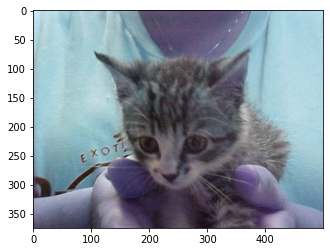
\includegraphics[width=0.48\textwidth]{Images/cat_1.png}
    \caption{Sample image from dataset.}
    \label{fig:sample-dataset}
\end{figure}

Image classification is where a computer can analyse an image and identify the ‘class’ the image falls under. (Or a probability of the image being part of a ‘class’.) A class is essentially a label, for instance, ‘car’, ‘animal’, ‘building’ and so on. 

This project aims to create multiple machine learning mdoels to predict if a photo given to the model is either a cat, or a dog. Three different network models were used to find the most efficient and accurate model for image classification.

